\documentclass{article}
\usepackage{graphicx}
\usepackage{float}
\usepackage{caption}
\usepackage{subcaption}
\usepackage{gensymb}
\usepackage[utf8]{inputenc}
\usepackage{amsmath}
\usepackage[a4paper, total={6in, 8in}]{geometry}

\renewcommand{\thesubsection}{\thesection.\alph{subsection}}

\begin{document}

\author{Antonella Dellanzo}
\title{Guía Convolución}
\date{}
\maketitle

Para realizar la convolución entre una imagen y su kernel, desarrollé un método llamado \textbf{convolucion} que toma como parámetros de entrada una imagen y un kernel. Las dimensiones de éste último pueden ser pares e impares, pero es requisito que sea una matriz cuadrada. De no serlo, se mostrará un mensaje de error.

Para realizar la convolución, me base en la fórmula propuesta en el libro de Rafael C. Gonzalez y Richard E. Woods\cite{libro}, la cual es:

\begin{equation}
w(x,y)\otimes f(x,y) = \sum_{s=-a}^{a} \sum_{t = -b}^{b} w(s,t)f(x-s,y-t)
\end{equation}

Como requiero que el kernel sea cuadrado, vale que $a=b$, con $a=\frac{n-1}{2}$. Además, dicha fórmula solo sirve para tamaños impares de kernel, por lo cual debí realizar una modificación en ella, iterando hasta $a+1$ cuando el tamaño del kernel es par. Luego obtengo:

\[   
w(x,y)\otimes f(x,y) := 
     \begin{cases}
        \sum_{s=-a}^{a} \sum_{t = -a}^{a} w(s,t)f(x-s,y-t) &\quad\text{si } mod(n,2) = mod(m,2) = 1\\
        \\
        \sum_{s=-a}^{a+1} \sum_{t = -a}^{a+1} w(s,t)f(x-s,y-t) &\quad\text{si } mod(n,2) = mod(m,2) = 0\\
     \end{cases}
\]

Para el ejercicio del enunciado, generé un método llamado \textbf{ejercicioConvolucion} que toma como parámetro de entrada una imagen y genera varias figuras, mostrando en cada una de ellas distintas convoluciones entre la imagen y uno de los 14 kernels del enunciado. Por ejemplo, para la imagen de lena se obtienen las siguientes figuras:

 \begin{figure}[H]
    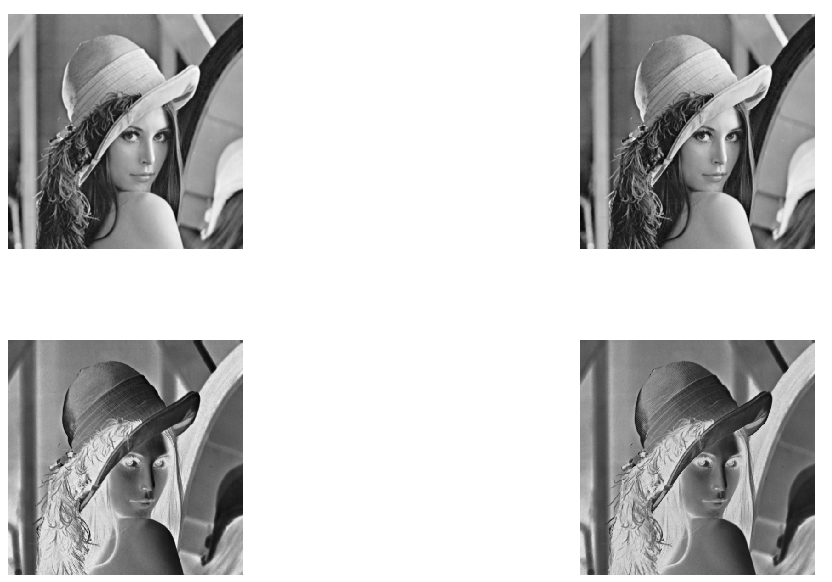
\includegraphics[width=0.9\textwidth]{figura1.png}
\end{figure}
 \begin{figure}[H]
    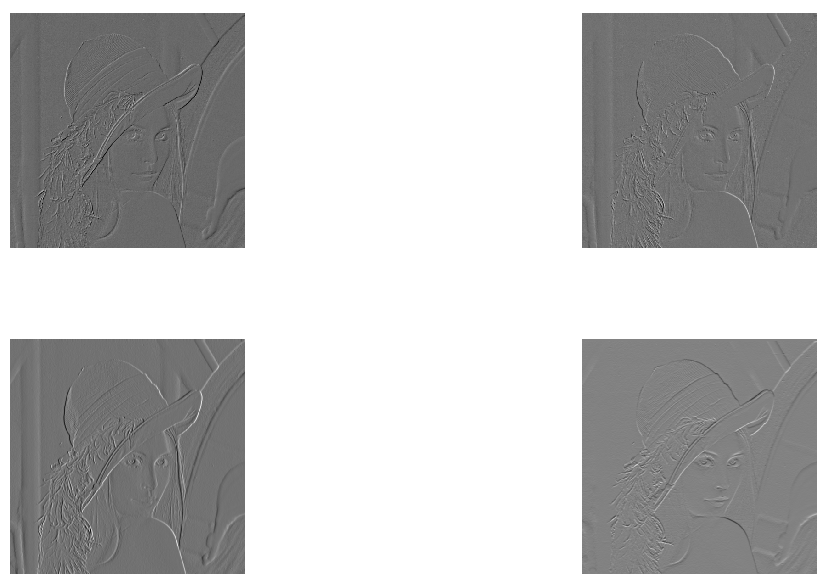
\includegraphics[width=0.9\textwidth]{figura2.png}
\end{figure}
 \begin{figure}[H]
    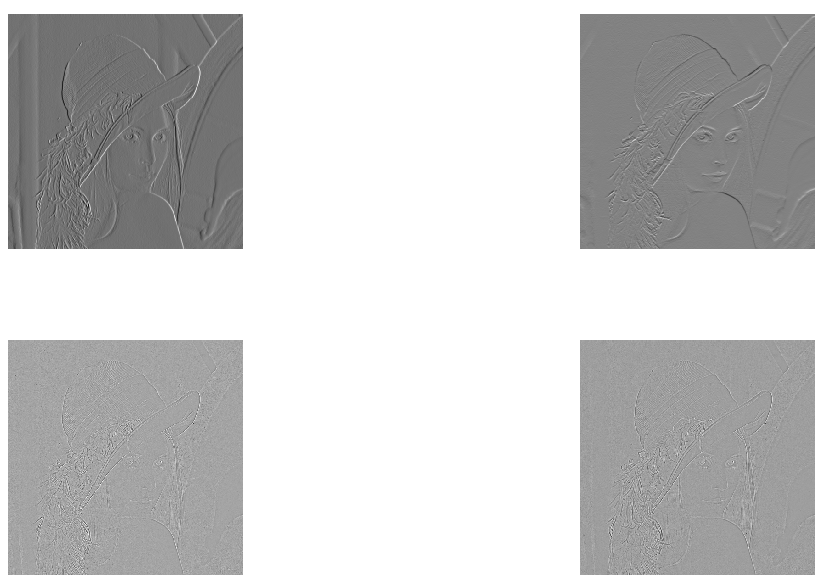
\includegraphics[width=0.9\textwidth]{figura3.png}
\end{figure}
 \begin{figure}[H]
    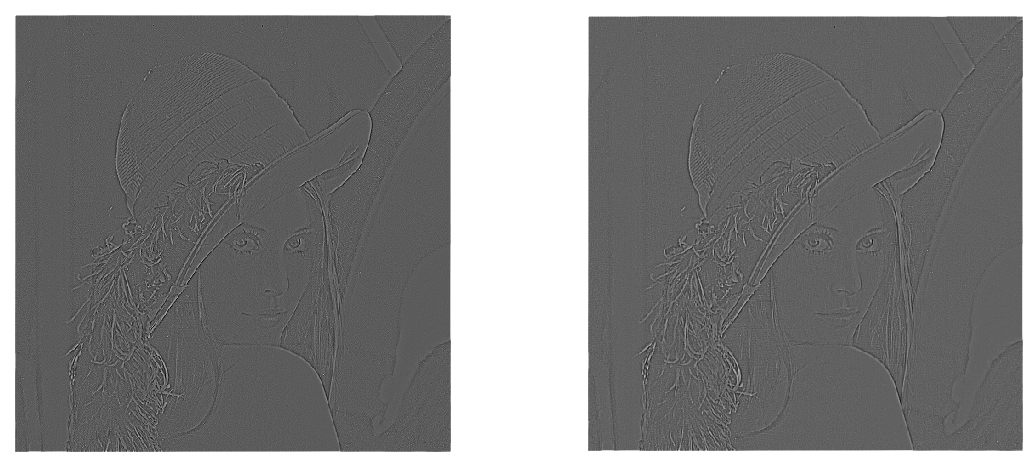
\includegraphics[width=0.9\textwidth]{figura4.png}
\end{figure}

\begin{thebibliography}{9}
\bibitem{libro}
Rafael C. Gonzalez and Richard Eugene Woods. \textit{Digital Image Processing.} 3rd Edition. Pearson Prentice Hall. 2007. ISBN-13: 978-0131687288.
\end{thebibliography}

\end{document}